\documentclass[aspectratio=169]{beamer}
\usepackage[utf8]{inputenc}
\usepackage{tikz}
\usepackage{tikz-cd}
\usepackage{tikz-layers}
\usepackage{pifont}
\usepackage{pgfpages}
\usepackage{pgfplots}
\usepackage{graphicx}
\usepackage[export]{adjustbox}
\usepackage{qrcode}
\usepackage{caption}
\usepackage{minted}
\usepackage[svgnames]{xcolor}
\usetikzlibrary{backgrounds}
\usetikzlibrary{decorations.pathreplacing}

% the drgtheme files live once at the repo root, in ../../../theme/
\makeatletter
\def\input@path{{../../../theme/}}
\makeatother
\graphicspath{{./images/}{../../../theme/}}

\usetheme{drgtheme}

%setup cover page variables
\title{MAC 233: External LED Lab}
\author{
    Dr Dan Brennan
}
\institute[UoS-DRG]{
    School of Mechanical, Aerospace, and Civil Engineering,\\
    University of Sheffield, UK
}
\date{MAC 233: \hspace{0.1em}\textbf{22/10/2025}}
%setup footer variables
\runninginstitute{MAC 233, School of MAC, University of Sheffield}
\email{d.s.brennan@sheffield.ac.uk}

%Begin Document
\begin{document}

%Create Title Page
\maketitle

\begin{frame}{MAC 233: Labs Overview}
    \begin{center}
        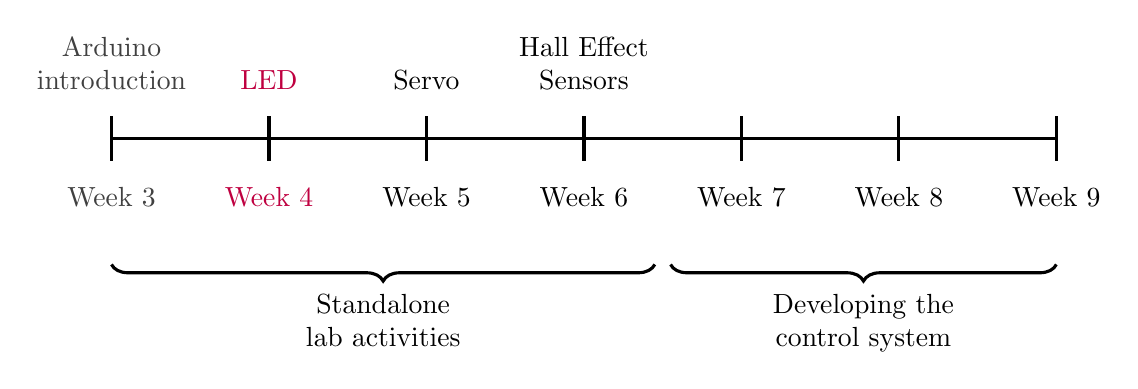
\begin{tikzpicture}[
            timeline/.style={color=black, line width=0.4mm},
            pastnode/.style={align=center, color=darkgray},
            currentnode/.style={align=center, color=purple},
            futurenode/.style={align=center, color=black}
        ]
            %line
            \draw[timeline] (-6, 0) -- (6, 0);

            % week ticks
            \foreach \x in {-6, -4, -2, 0, 2, 4, 6}{
                \draw[timeline] (\x, -0.28) -- (\x, 0.28);
            }

            % weeks (below the line)
            \node[pastnode, below] at (-6, -0.5) {Week 3};
            \node[currentnode, below] at (-4, -0.5) {Week 4};
            \node[futurenode, below] at (-2, -0.5) {Week 5};
            \node[futurenode, below] at (0, -0.5) {Week 6};
            \node[futurenode, below] at (2, -0.5) {Week 7};
            \node[futurenode, below] at (4, -0.5) {Week 8};
            \node[futurenode, below] at (6, -0.5) {Week 9};

            % activities (above the line)
            \node[pastnode, above] at (-6, 0.5) {Arduino\\introduction};
            \node[currentnode, above] at (-4, 0.5) {LED};
            \node[futurenode, above] at (-2, 0.5) {Servo};
            \node[futurenode, above] at (0, 0.5) {Hall Effect\\Sensors};

            % phases
            \draw[timeline, decorate, decoration={brace, amplitude=6pt, mirror}] (-6, -1.6) -- (0.9, -1.6);
            \node[futurenode, below] at (-2.55, -1.85) {Standalone\\lab activities};
            \draw[timeline, decorate, decoration={brace, amplitude=6pt, mirror}] (1.1, -1.6) -- (6, -1.6);
            \node[futurenode, below] at (3.55, -1.85) {Developing the \\ control system};

        \end{tikzpicture}
    \end{center}
\end{frame}

\begin{frame}{Variables: Scope}
    \Large
    \inputminted{arduino}{./src/arduino-scope.txt}
\end{frame}

\begin{frame}{Today's Lab: Prerequisites}
    \Large
    This worksheet builds upon the Lab 1 worksheet. You will have needed to complete the Lab 1 worksheet before you can continue with this lab.\\
    
    Out of your Arduino pack, you will need: 1 Arduino, 1 breadboard, 1 LED, 1 $220\Omega$ resistor, and 1 jumper cable.
\end{frame}

\begin{frame}{Today's Lab: Objectives}
    \Large
    The objective of today's lab is to learn how to use an electronic breadboard to create a circuit and to control an external output on the Arduino.\\

    We will be taking the scenario from the previous worksheet and changing it to communicate with an external LED.
\end{frame}

\begin{frame}{Lab 2: External LED}
    \begin{center}
        Login to Blackboard: \url{https://vle.shef.ac.uk/}
        \begin{tikzpicture}[
            highlight/.style={draw=purple, line width=.25mm},
        ]
            % screenshot
            \node[] at (0, 0) {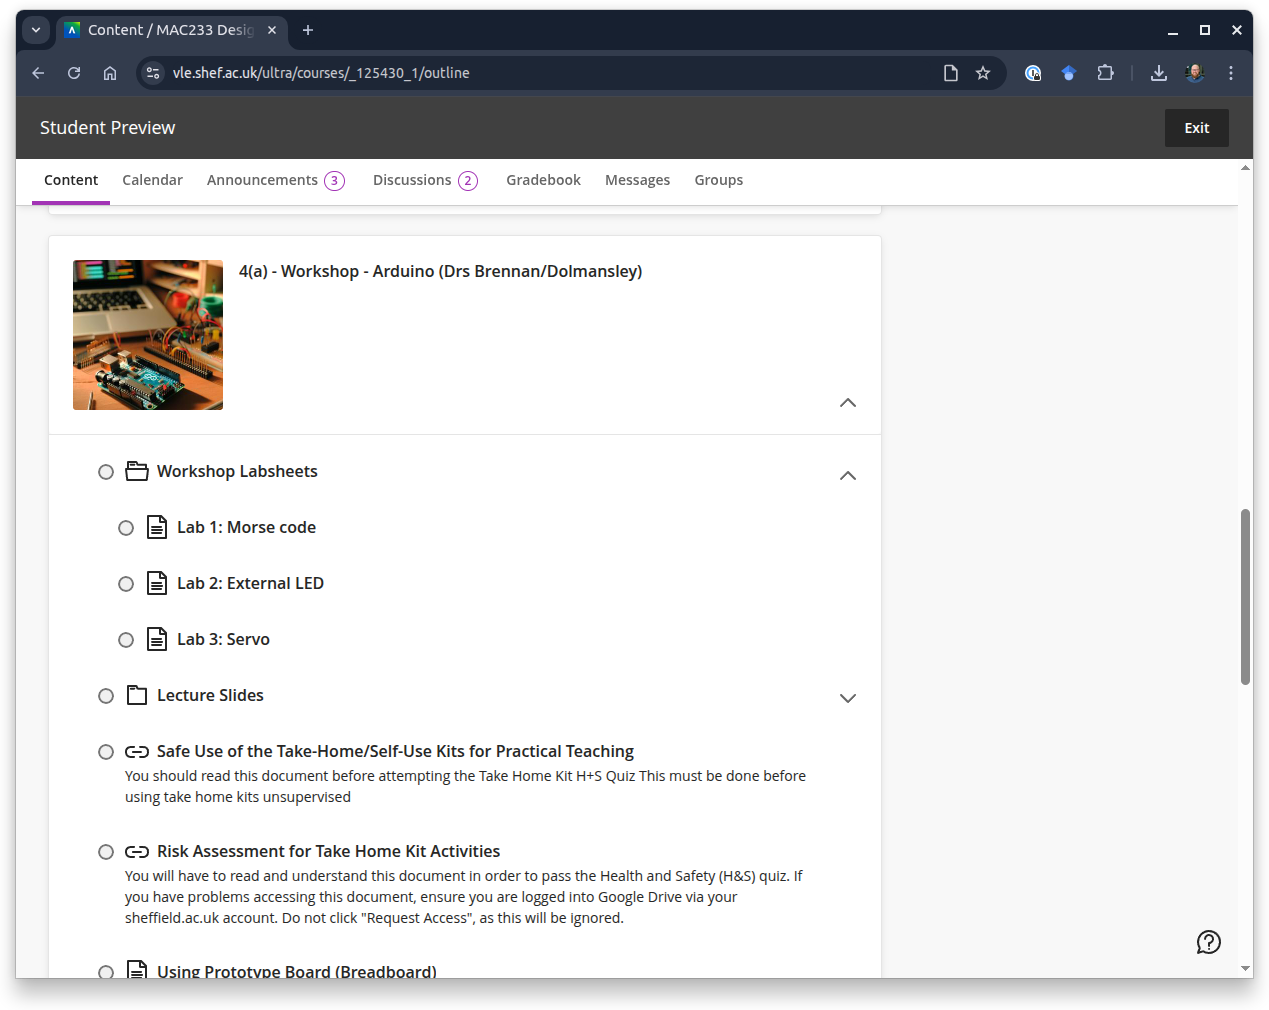
\includegraphics[width=.7\textwidth]{./images/lab-2.png}};
            % highlight
            \draw[highlight] (-4.15, -.825) rectangle ++(2, 0.4);
        \end{tikzpicture}
    \end{center}
\end{frame}

\begin{frame}{Wiring Diagram}
    \vspace{-.5em}
    \begin{center}
        \begin{tikzpicture}[
            scale=1.65, transform shape, rotate=90,
            wire/.style={line width=.8mm},
            leg/.style={draw=DimGray},
            jumper/.style={draw=LimeGreen},
        ]

            %% legs 5 per span y = 0.188, per span x = 0.183
            \draw[wire, leg] (.975,-0.515) -- (.975, 0.792);
            \draw[wire, leg] (.792,-1.61) -- (.792, -0.49);

            %% cables
            \draw[wire, jumper] (.607,-1.61) -- (.607, 0.604);

            %% components
            \filldraw[fill=red, draw=black] (.79,-1.05) circle (1.25mm);
            \node[] at (.975, 0.14) {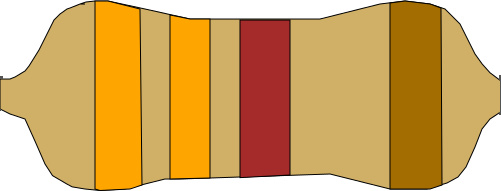
\includegraphics[angle=90, origin=c,width=1.75mm]{./images/resistor-220.png}};
            \node[] at (-.13, 1.43) {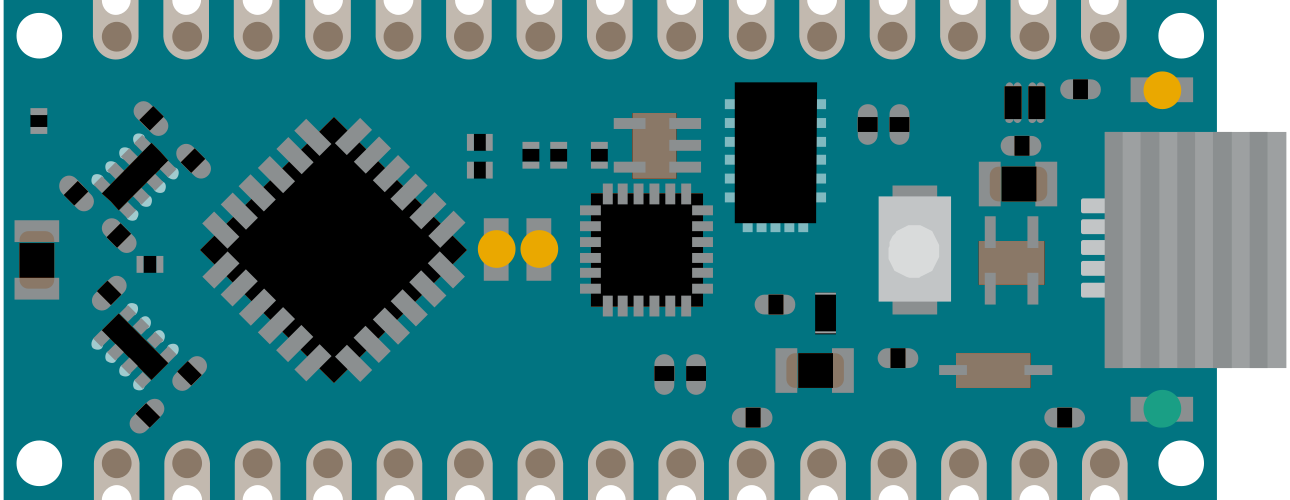
\includegraphics[angle=90, origin=c, width=3.38em]{./images/nano.png}};

            %% breadboard background
            \begin{scope}[on background layer]
                \node[] at (0, 0) {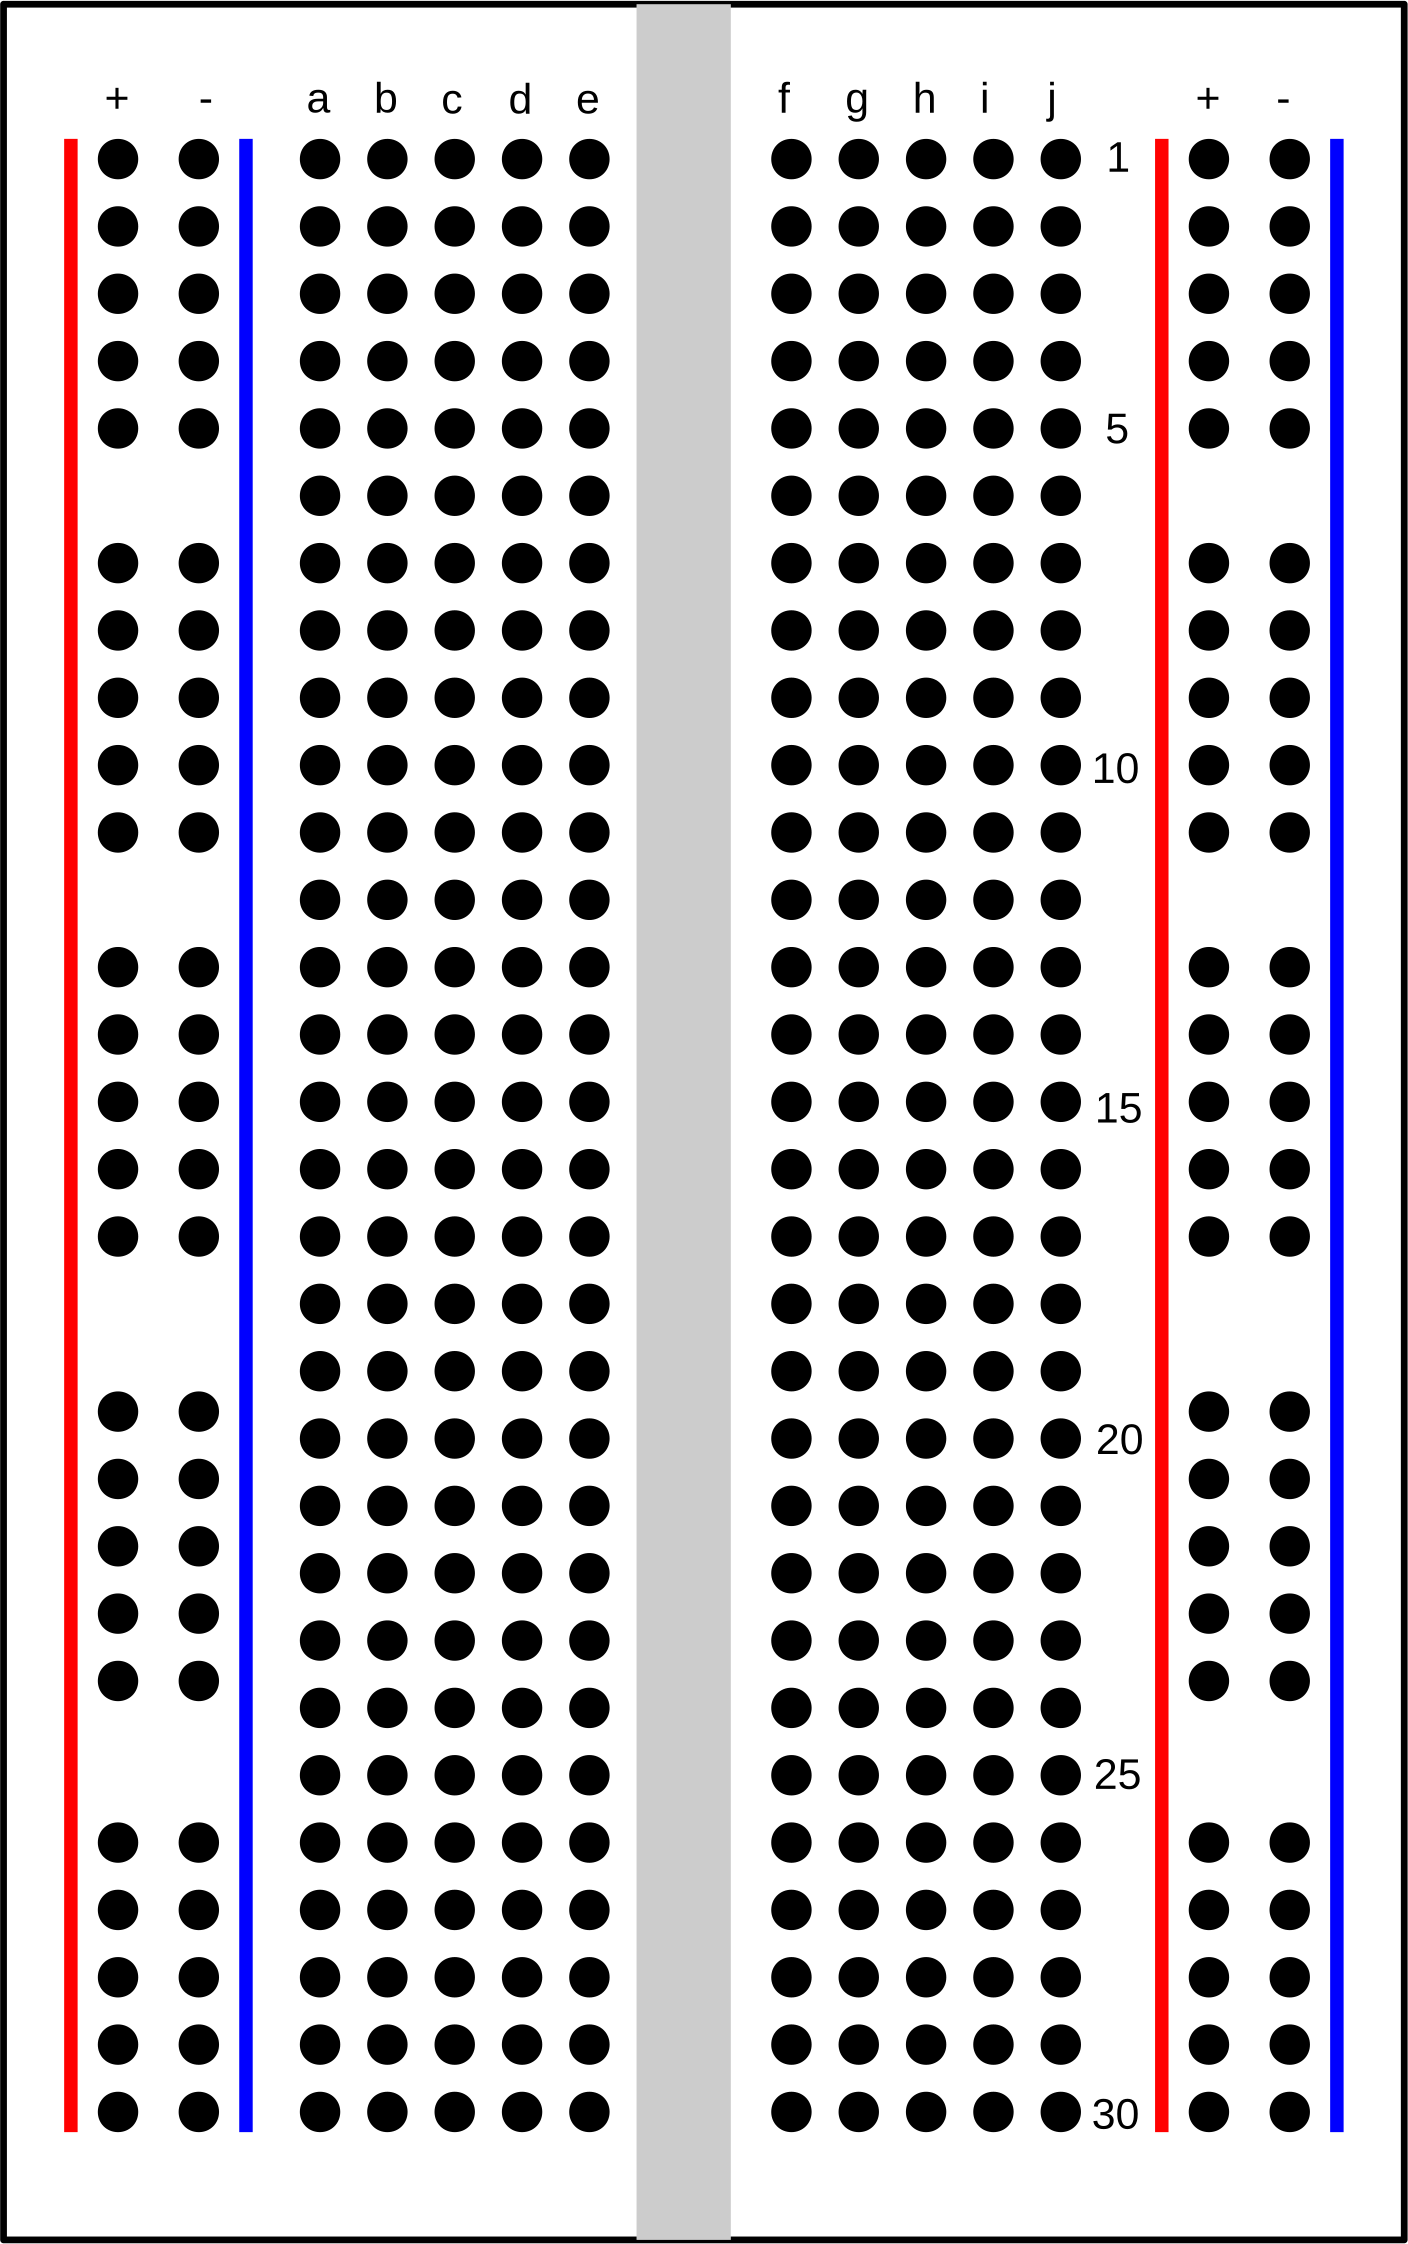
\includegraphics[width=10em]{./images/breadboard.png}};
            \end{scope}

        \end{tikzpicture}
    \end{center}
    \tiny
    Breadboard source: \url{https://freesvg.org/breadboard}, Resistor source \url{https://freesvg.org/resistor-330-ohm}.
\end{frame}

\end{document}
